\documentclass[12pt]{beamer}
\usetheme{Boadilla}
\usepackage{graphicx}
\usepackage{algorithm2e}
\graphicspath{{images/}}
\title{CMPT 155: Computer Applications for Life Sciences}
\subtitle{Lecture 7: Formulas and Functions (Part 3)}
\author{Ivan E. Perez}
\institute{}
\date{February 11, 2022}
\usepackage{booktabs} % Allows the use of \toprule, 
\usepackage{appendix}
\usepackage{enumerate,multicol}
\usepackage{amsmath, amssymb, amsthm}
\usepackage{tikz}
\usepackage{amsxtra}
\begin{document}
	
	\begin{frame}
		\titlepage
	\end{frame}
	
	\begin{frame}
		\frametitle{Presentation Outline}
		\tableofcontents
	\end{frame}
	\section{Homework \& Administrative}
	
	\begin{frame}
		\frametitle{Homework \& Administrative Schedule}
		\begin{itemize}
			\item Homework 2 Due: Tuesday, February $22^{\text{nd}}$ at 6pm
			\item Homework 3 Due: Tuesday, March $1^{\text{st}}$ at 6pm
			\item First Midterm Review:  Wednesday, March $2^{\text{nd}}$
			\item First Midterm Exam: Friday, March, $4^{\text{th}}$
			
		\end{itemize}
	\end{frame}
\section{Range Functions: MEDIAN, MAX/MIN, LARGE/SMALL}
	\begin{frame}
		\frametitle{MEDIAN()}
		\begin{itemize}
			\item The Median of a set of numbers is the middle number. 
			\item	example: given a sequence of numbers 1,2,4,12,15. the median is the middle number. where middle means that there are equal elements before and after the number. 
		\end{itemize}
		\begin{figure}[htb]
	\begin{minipage}[t]{0.5\linewidth}\centering
		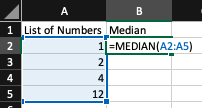
\includegraphics[width=0.9\linewidth]{MEDIAN_even.png}
		\medskip
		\centerline{(a)}
	\end{minipage}\hfill
	\begin{minipage}[t]{0.5\linewidth}\centering
		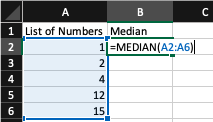
\includegraphics[width=0.9\linewidth]{MEDIAN_odd.png}
		\medskip
		\centerline{(b)}
	\end{minipage}
\end{figure}
Try running these functions and seeing what median you return!
	\end{frame}
	\begin{frame}
		\frametitle{MAX() and MIN()}
			MAX()
			\begin{itemize}
				\item inputs:
				\begin{itemize}
					\item \texttt{[number1], [number2], \ldots}
					\item selection of or single cells containing numerics.
				\end{itemize}
				\item ouptuts:
				\begin{itemize}
					\item single value denoting the\textbf{ maximum value} from the selection.
				\end{itemize}
		\end{itemize}
		MIN() 
			\begin{itemize}
			\item inputs:
			\begin{itemize}
				\item \texttt{[number1], [number2], \ldots}
				\item selection of cells or single cells containing numerics. 
			\end{itemize}
			\item ouptuts:
			\begin{itemize}
				\item single value denoting the\textbf{ minimum value} from the selection.
			\end{itemize}
	\end{itemize}
	% things to do in this slide
	% images 
	\end{frame}
	\begin{frame}
		\frametitle{LARGE() and SMALL()}
		We can use Large and small to return the ordinally largest/smallest values from a selection of numerics. \\
		LARGE(range, position)
		\begin{itemize}
			\item inputs
			\begin{itemize}
				\item \texttt{array} : selection of cells that contain numerics
				\item \texttt{k}: integer that denotes fist, second, \ldots, $\texttt{k}^{\text{th}}$ highest in the list.
			\end{itemize}
			\item returns:
				\begin{itemize}
					\item value from the selection that is the $\texttt{k}^{\text{th}}$ highest from the maximum value. 
				\end{itemize}
		\end{itemize}
		SMALL (range, position)
			\begin{itemize}
				\item inputs
				\begin{itemize}
					\item \texttt{array} : selection of cells that contain numerics
					\item \texttt{k}: integer that denotes fist, second, \ldots, $\texttt{k}^{\text{th}}$ lowest in the list.
				\end{itemize}
				\item returns:
				\begin{itemize}
					\item value from the selection that is the $\texttt{k}^{\text{th}}$ lowest from the minimum value. 
				\end{itemize}
			\end{itemize}	
	\end{frame}
\begin{frame}
	\frametitle{Exercise 1: Student Grades redux}
	\begin{enumerate}
		\item Download \textit{StudentGrades2.xlsx}
		\item Use the functions we learned to add following statistics found at the bottom of the table:
		\begin{itemize}
			\item Total
			\item Average
			\item Median
			\item Highest Score
			\item Second Highest Score
			\item Third Highest Score 
			\item Lowest Score
		\end{itemize}
	\end{enumerate} 
	\end{frame}
\begin{frame}
	\frametitle{Exercise 1: Solution}
	\begin{enumerate}
		\item See Lecture 06 for solutions to get Weighted Averages entered in Cells \texttt{E2:E10}
		\item to get Total use SUM() on cells \texttt{E2:E10}
		\item to get Average use AVERAGE() on cells \texttt{E2:E10}
		\item to get Median use MEDIAN() on cells \texttt{E2:E10}
		\item to get Highest Score use MAX() on cells \texttt{E2:E10}
		\item to get Second Highest Score use LARGE() pass use \texttt{E2:10} in \texttt{array} and 2 as \texttt{k}
		\item to get Third Highest Score use LARGE() pass use \texttt{E2:10} in \texttt{array} and 3 as \texttt{k}
		item to get Loewst Score use MIN() on cells \texttt{E2:E10}
	\end{enumerate}
\end{frame}
\begin{frame}
	\frametitle{Exercise 1: Solution (continued)}
	\begin{center}
		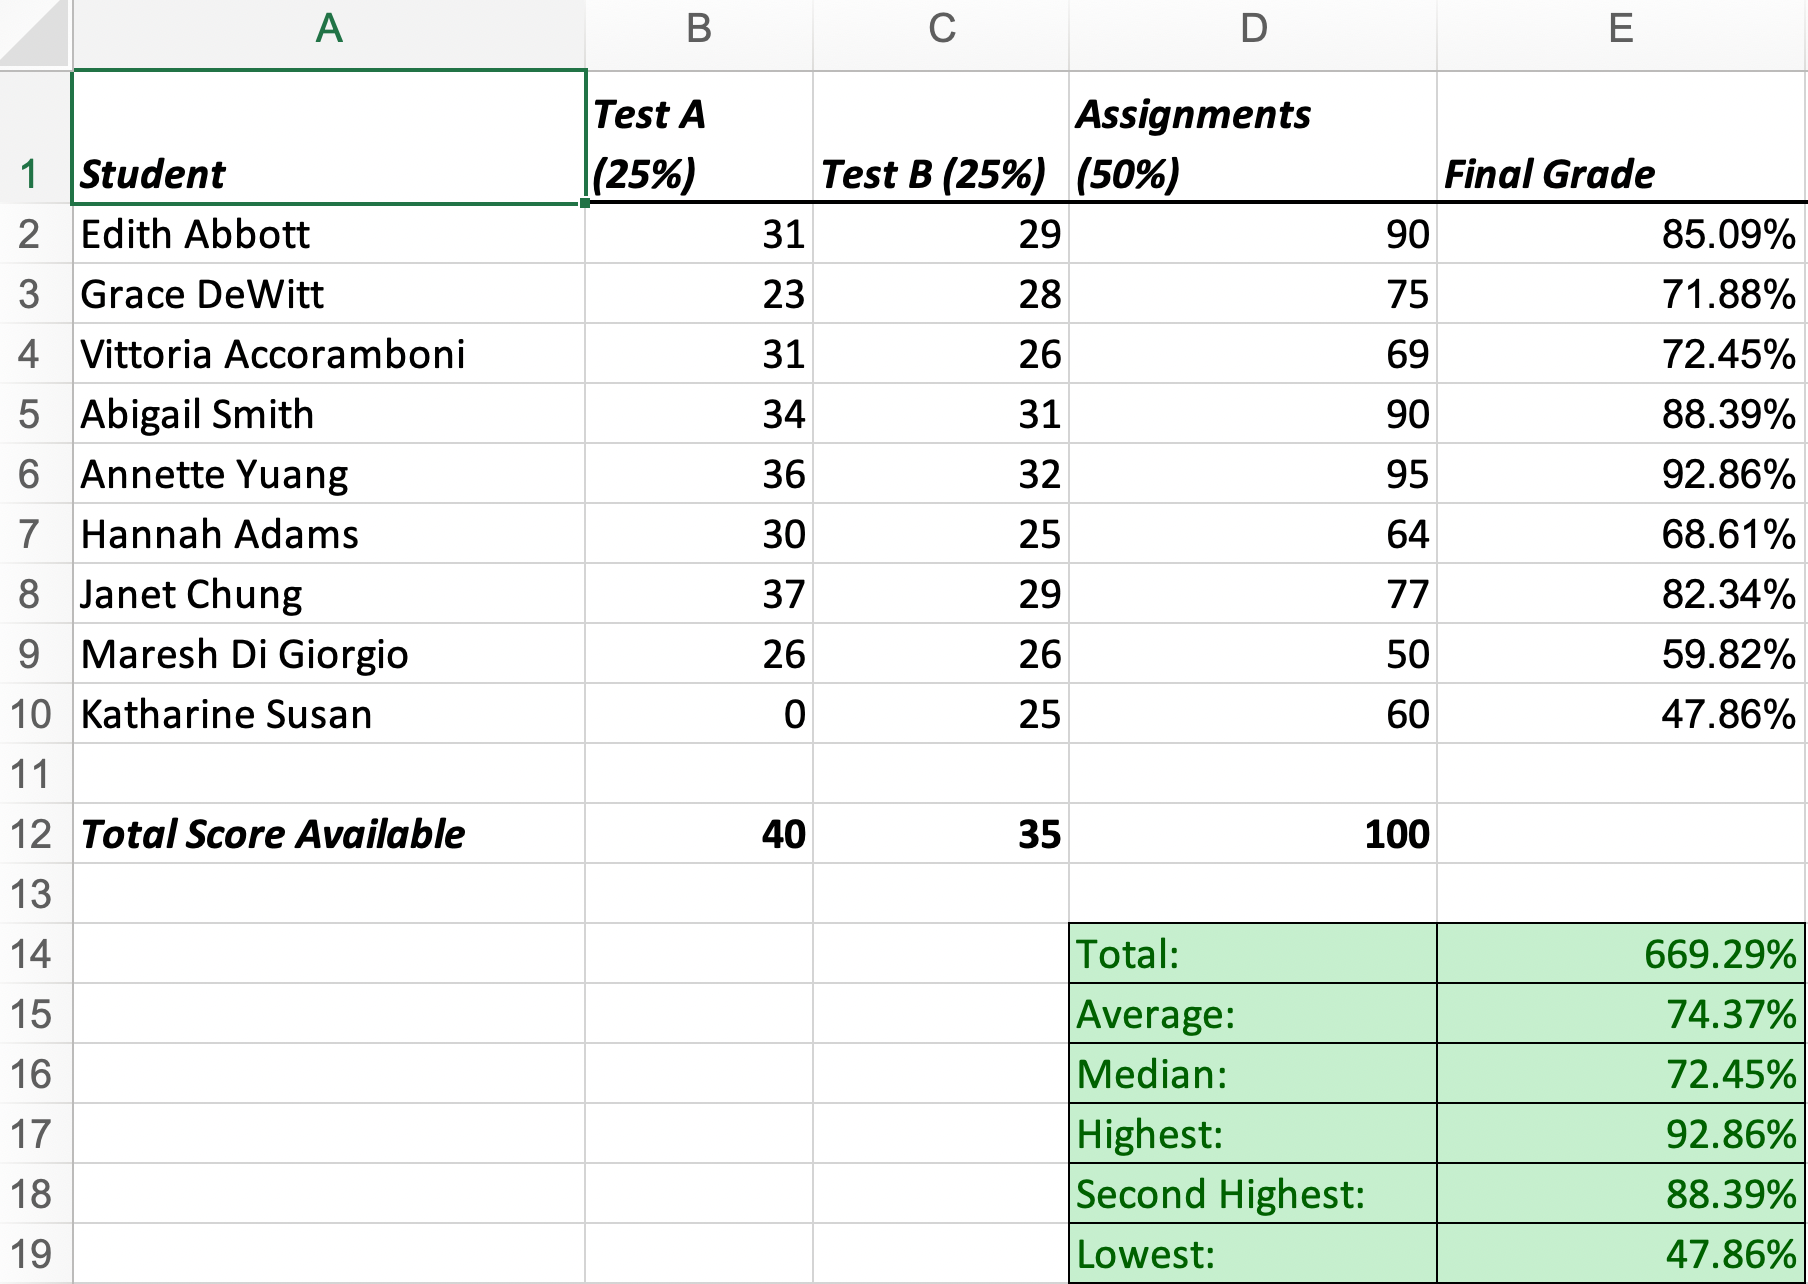
\includegraphics[width=0.9\textwidth]{StudentGrades2Soln.png}
	\end{center}
\end{frame}
\section{Value Functions: ABS, ROUND, RAND}
\begin{frame}
	\frametitle{ABS() and ROUND()}
	ABS: 
		\begin{itemize}
			\item The Absolute value function returns the absolute value of a numeric value passed
			\item inputs : \texttt{number} 
			\item returns : numeric value 
			\item Notes: Is there a way to make ABS() using IF()?
		\end{itemize}
	ROUND():
			\begin{itemize}
				\item rounds a numeric value to whatever level of precision you choose.
				\item inputs :
				\begin{itemize}
					\item \texttt{number\_to\_round}: Numeric value you would like to round
					\item \texttt{number\_of\_digits}: Number of digits function is rounding to.  
				\end{itemize}
			\end{itemize}
	
	\begin{figure}[htb]
		\begin{minipage}[t]{0.5\linewidth}\centering
			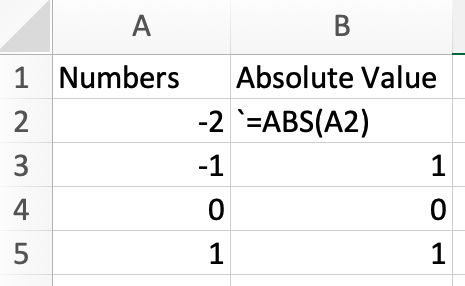
\includegraphics[width=0.5\linewidth]{ABS.png}
			\medskip
			\centerline{(a)}
		\end{minipage}\hfill
		\begin{minipage}[t]{0.5\linewidth}\centering
			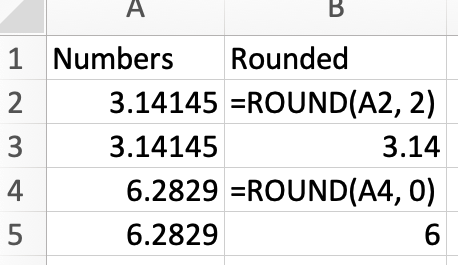
\includegraphics[width=0.5\linewidth]{ROUND.png}
			\medskip
			\centerline{(b)}
		\end{minipage}
	\end{figure}
\end{frame}

\begin{frame}
\frametitle{RAND()}
 RAND()
\begin{itemize}
	\item gives you a random fractional number that is less than 1, but greater than or equal to 0.
	\begin{itemize}
		\item inputs : None
		\item returns : Numeric value between 0 and 1
	\end{itemize}
\end{itemize}\bigskip
	Things to Consider...\\
	How would I:
	\begin{itemize}
		\item generate a random whole number between 0 and 10?
		\item generate a random whole number between 0 and 100?
	\end{itemize}

\end{frame}
\section{Counting Functions: COUNT, COUNTA, COUNTBLANK, COUNTIF}
\begin{frame}
	\frametitle{COUNT(), COUNTA(), COUNTBLANK()}
	COUNT(), COUNTA(), COUNTBLANK()
		\begin{itemize}
			\item inputs : \texttt{number1, number2, \ldots}
			\item returns : 
			\begin{itemize}
				\item for COUNT() $\rightarrow$ number of cells that contain numerics.
				\item for COUNTA() $\rightarrow$ number of cells that contain \textbf{any} information.
				\item for COUNTBLANK() $\rightarrow$ number of empty/\textbf{blank} cells.
			\end{itemize}
		\end{itemize}
\end{frame}

\begin{frame}
	\frametitle{COUNTIF()}
		Returns the number of cells that satisfy the logical criteria given.
		\begin{itemize}
			\item inputs :
			\begin{itemize}
				\item \texttt{range} : cell range to look over
				\item \texttt{criteria} : criteria/logical argument that must be satisfied 
			\end{itemize}
			\item returns : integer number of cells that satisfy logical argument. 
		\end{itemize}
\end{frame}
\begin{frame}
	\frametitle{COUNT Example}
	\begin{figure}
		\begin{center}
			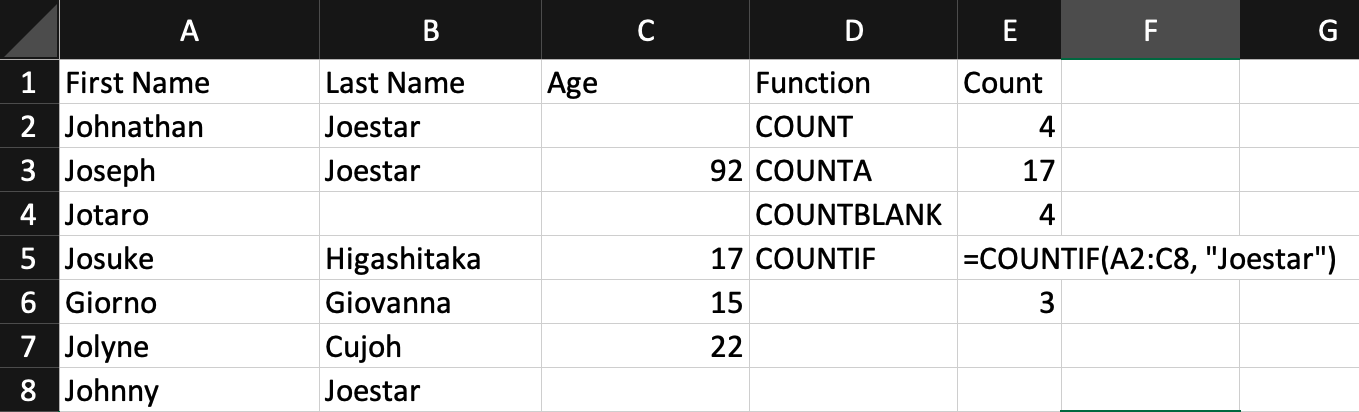
\includegraphics[width=0.9\textwidth]{COUNTEXAMPLE.png}
			\caption{Example of COUNT(), COUNTA(), COUNTBLANK(), COUNTIF() applied over cells A2:C8}
	\end{center}
	\end{figure}
\end{frame}
\begin{frame}
	\frametitle{Exercise 2: Fruit Purchases \textit{redux revival}}
	\begin{enumerate}
		\item Download \textit{Fruit\_Purcases.xlsx}
		\item Redo the fruit counting exercise using the counting functions (COUNT, COUNTA, COUNTIF)
	\end{enumerate}
\end{frame}
\begin{frame}
	\frametitle{Exercise 2: Solution}
	\begin{enumerate}
		\item For each fruit (apples, kiwi, pear) write a COUNTIF statement that takes a \texttt{range} = B3:B20,
		and a logical argument as the fruit in quotation marks.
		\item In cells B22, B23, B24 you can write out 
			\begin{itemize}
				\item B22 : \texttt{=COUNTIF(B3:B20, "apples")}
				\item B23 : \texttt{=COUNTIF(B3:B20, "kiwi")}
				\item B24 : \texttt{=COUNTIF(B3:B20, "pears")}
			\end{itemize}
	\end{enumerate}
	\begin{center}
		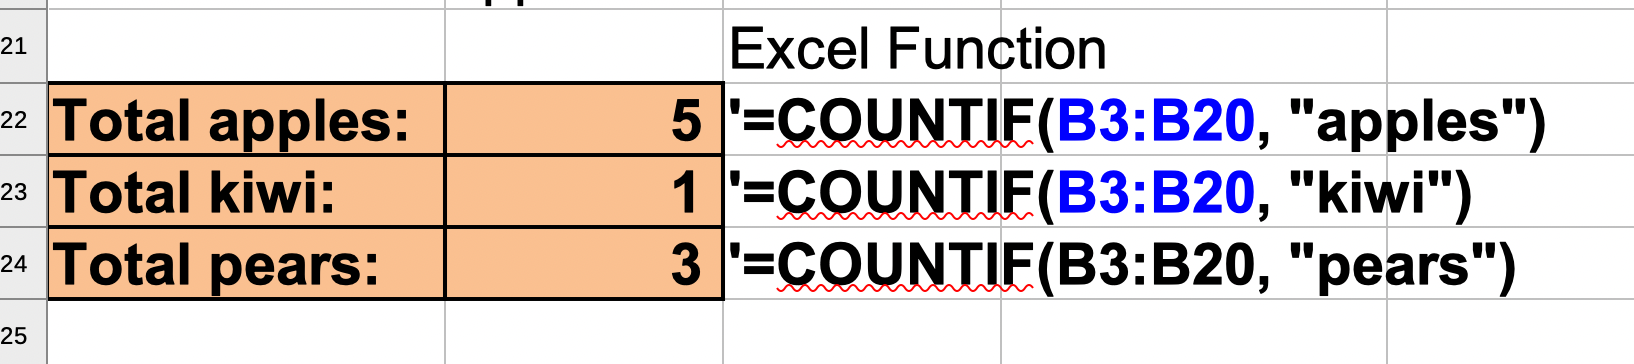
\includegraphics[width = 0.9\textwidth ]{FruitsReduxRevival.png}
	\end{center}
\end{frame}

\section{VLOOKUP}
\begin{frame}
	\frametitle{VLOOKUP}
	\begin{itemize}
		\item returns something.
		\item inputs : 
			\begin{itemize}
				\item \texttt{lookup\_value} : cell reference\\
				Your query (i.e., What it is you are looking for.) 
				\item \texttt{range} : cell range\\
				The range of data you are looking in that contains \texttt{lookup\_value}.
				\item \texttt{column\_index\_number} : integer\\
				The column index starting from 1 that you want to display/retrieve.
				\item \texttt{FALSE} : FALSE\\ if exact match is needed, TRUE if close enough is okay.
			\end{itemize}
		\end{itemize}
\end{frame}
\begin{frame}
	\frametitle{VLOOKUP Example}
	\begin{enumerate}
	\item Download \textit{VLookupExample.xlsx} from moodle.
	\item Fill out cells \texttt{C4:C8} using the appropriate VLOOKUP function call, for each search field given a search term in cell \texttt{B2}. 
	\item For Example: If we enter \texttt{1} for the product ID in cell \texttt{B2},\\  then out VLOOKUP arguments for \textbf{Product} are:
		\begin{tabular}{l l }
		 	\texttt{look\_up\_value : B3}& $\leftarrow$ This is our search term.\\
		 	\texttt{range : A12:F78}& $\leftarrow$  The entire dataset.\\
		 	\texttt{column\_index\_number : 2} &$\leftarrow$ We want the second column.\\
		 	\texttt{FALSE : FALSE}& $\leftarrow$ We want \textbf{exact matches}.\\
		 \end{tabular}

	 	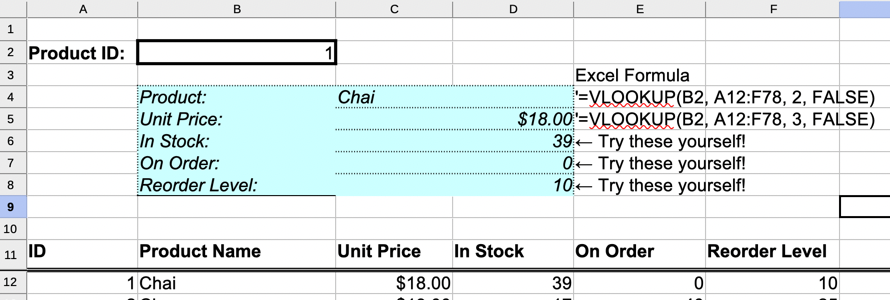
\includegraphics[width =0.9\textwidth ]{VLOOKUPEx.png}
	\end{enumerate}
\end{frame}
\begin{frame}
	\frametitle{Exercise 3: Student Grades 4}
	\begin{enumerate}
		\item Download \textit{StudentGrades4.xlsx}
		\item Compute the average for each student.
		\item Use VLOOKUP to assign letter grades(Grade) and grade points(QPts) based on the computed average.
		\item Write whether the students Passed or Failed in the comments section. 
		\item Count the number of students that passed and failed. 
	\end{enumerate}
\end{frame}
\begin{frame}
	\frametitle{Exercise 3: Solution}
	\begin{enumerate}
		\item In cell D2, compute the average for the first cell by typing
		\begin{itemize}
			\item  \texttt{=AVERAGE(A2:C2)}
		\end{itemize}
		\item Use Autofill to assign averages for from D2:D10.
		\item In Cell E2, use VLOOKUP to assign grades. The arguments are:
			\begin{tabular}{l l }
				\texttt{look\_up\_value : D2}& $\leftarrow$ This is our search term.\\
				\texttt{range : \$C\$17:\$D\$21}& $\leftarrow$ `Averages' \& `Grade' columns.\\
				\texttt{column\_index\_number : 2} &$\leftarrow$ We want the `Grade' column.\\
				\texttt{FALSE : True}& $\leftarrow$ for \textbf{approximate matches}.\\
			\end{tabular}
		\item Use Autofill to assign further grades
	\end{enumerate}
\end{frame}
\begin{frame}
	\frametitle{Exercise 3: Solution (continued)}
	\begin{enumerate}
		\setcounter{enumi}{4}
		\item In Cell F2, use VLOOKUP to assign grade points `QPts'.\\ The arguments are:
		\begin{tabular}{l l }
			\texttt{look\_up\_value : E2}& $\leftarrow$ This is our search term.\\
			\texttt{range : \$D\$17:\$E\$21}& $\leftarrow$ `Grade' \& `QPts' columns.\\
			\texttt{column\_index\_number : 2} &$\leftarrow$ We want the `QPts' column.\\
			\texttt{FALSE : FALSE}& $\leftarrow$ for \textbf{exact matches}.\\
		\end{tabular}
		\item Use Autofill to assign further grade points
	\end{enumerate}
\end{frame}
\begin{frame}
	\frametitle{Exercise 3: Solution (continued)}
		\begin{enumerate}
			\setcounter{enumi}{6}
			\item In Cell G2 use IF() to show ``Pass" if a student passed and ``Fail" if a student failed.
			\begin{itemize}
				\item We can use The `QPts' column to help us determine whether a student passed.
				\item If a student earned \textbf{strictly less} than 2 QPts then they did not pass the course.
				\item Cell G2 Should read \texttt{=IF(F3<2, "Fail", "Pass")} 
				\item Autofill for the following cells in the column.
			\end{itemize}
		\item In Cell C12 use COUNTIF() to count only the students who have the comment "Passed".
			\begin{itemize}
				\item Cell C12 Should Read: \texttt{=COUNTIF("Passed", G2:G10)}
			\end{itemize}
		\item In Cell C12 use COUNTIF() to count only the students who have the comment "Passed".
		\begin{itemize}
			\item Cell C13 Should Read: \texttt{=COUNTIF("Failed", G2:G10)}
		\end{itemize}
		\end{enumerate}
\end{frame}

\begin{frame}
	\frametitle{Exercise 3: Solution (continued)}
		\begin{center}
			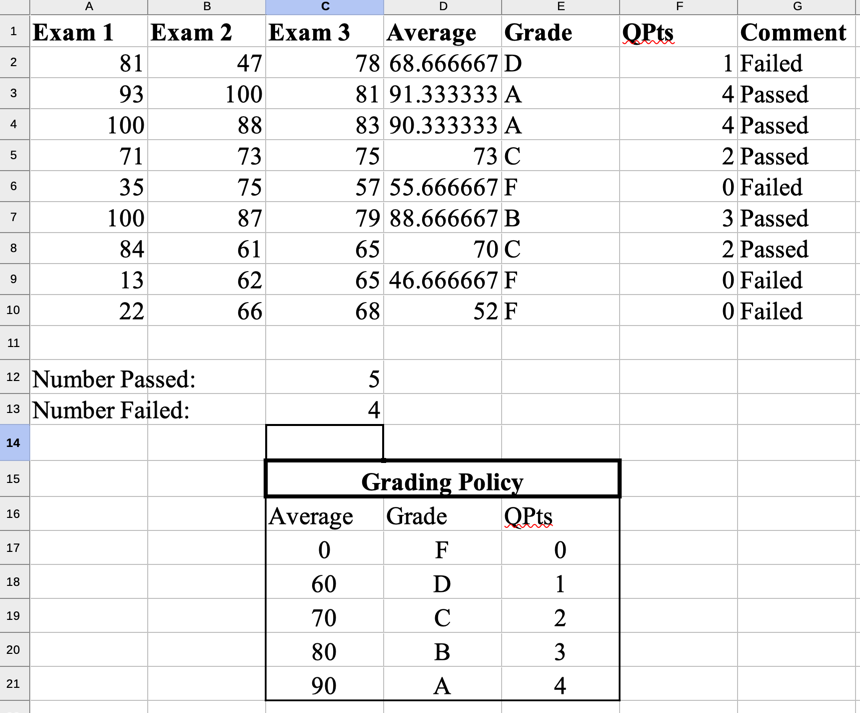
\includegraphics[width= 0.8 \textwidth]{Exercise3Soln}
		\end{center}
	
\end{frame}	
\begin{frame}
	\frametitle{Further Reading}
	Computer Applications for Life Sciences Chapter 1 p. 1-14, 
	covers lectures 4-7. 
\end{frame}	
\end{document}
